% !TEX root = resilience.tex
% ACM CoNEXT 2026 submission: single-column acmsmall, double-anonymous review.
% Bundled acmart.cls is v1.48 (2017). Replace with a recent CTAN acmart
% (>= v1.85) before camera-ready; v1.48 supports acmsmall+anonymous+review
% and is fine for the review draft.
\documentclass[acmsmall,anonymous,review,nonacm,10pt]{acmart}

\setcopyright{none}
\settopmatter{printacmref=false,printccs=false,printfolios=true}
\acmConference[CoNEXT '26]{ACM CoNEXT 2026}{December 2026}{Utrecht, The Netherlands}
\bibliographystyle{ACM-Reference-Format}

\input{packages}
\input{macros}

\title{SCULPTOR Has Your Back(up Path): Carving Interdomain
       Routes to Services}

\ifisanon
\author{Anonymous Submission \# 950}
\affiliation{\institution{}\country{}}
\else
\author{Thomas Koch}
\affiliation{\institution{Columbia University}\country{USA}}
\author{Ilgar Mammadov}
\affiliation{\institution{Columbia University}\country{USA}}
\author{Ethan Katz-Bassett}
\affiliation{\institution{Columbia University}\country{USA}}
\author{Sharad Agarwal}
\affiliation{\institution{Microsoft}\country{USA}}
\fi

\begin{document}

\begin{abstract}
Cloud and content providers (\servprods) serve diverse Internet
applications --- enterprise services, gaming, video, real-time
AI inference --- with goals that pull in different directions:
low latency for some flows, high availability for others, low cost
for bulk transfers, and graceful behavior when peering links fail
or flash crowds arrive.  Today's interdomain routing primitives
force \servprods to pick \emph{one} goal: anycast for availability,
unicast for latency, manual reroutes for failures, or static
overprovisioning for capacity.  Existing proactive systems such
as \painter and \anyopt improve on this for a \emph{single}
objective (steady-state latency), but their objective-specific
search procedures do not generalize.

We present \sparse, a framework that proactively computes BGP
ingress advertisements jointly optimizing arbitrary combinations
of latency, capacity, cost, and resilience objectives.  \sparse
treats path performance as a black box: it learns a probabilistic
model of how user groups route by issuing a handful of test
advertisements, and uses gradient descent over a continuous
relaxation of advertisement configurations to navigate a search
space of more than $2^{10{,}000}$ possibilities.  We prototype
\sparse on the PEERING testbed running over Vultr's public cloud
(32~sites, ${>}10{,}000$ peerings) and evaluate on the real
Internet via RIPE Atlas.  Compared with \painter, \sparse keeps
latency within $2.0$\,ms of an unrealizable per-peering optimum
(vs.\ $5.5$\,ms for \painter), absorbs $41\%$ less link overload
during site failures, sustains a $3\times$ larger flash crowd on
the same infrastructure, halves the congestion experienced by
high-priority flows, and lowers traffic cost by up to
$3\times$ closer to optimal.  \sparse is the first general-purpose,
proactive framework for multi-objective interdomain ingress
traffic engineering.
\end{abstract}

\maketitle

%==============================================================
\section{Introduction}
\label{sec:intro}

\servprods host services that are increasingly performance- and
availability-sensitive: enterprise applications with strict SLAs
\cite{painter,saving-private-wan}; gaming and AR/VR that demand
$\leq$\,10\,ms latency and $\leq$\,3\,ms jitter
\cite{latency-shears,vr-jitter-test}; large model inference and
video uploads whose request payloads now look more like CDN
\emph{ingress} than the small TCP acknowledgements of a decade ago
\cite{google-cloud-video-ai,microsoft-cloud-video-ai}.  These
services share the same underlying network and frequently experience
the same incidents --- DDoS attacks, peering disputes, link
failures, flash crowds --- that can simultaneously overload one
ingress and leave a backup site idle
\cite{moura2016anycast,ixp-scrubber,increasing-ddos-siliconangle,fastroute,tipsy,dhamdhere2018inferring}.
A modern \servprod therefore needs a routing strategy that
\emph{jointly} satisfies multiple, often conflicting, objectives:
latency, capacity, cost, and resilience to unexpected events.

Today's interdomain primitives do not provide one.  BGP exposes
exactly one ingress per destination prefix to each source AS, so
\servprods must choose, once, between (a)~\emph{anycast},
which prioritises availability at the cost of fine-grained
latency control \cite{tom-anycast,jiangchen-cdn-imc,regional-anycast};
(b)~\emph{unicast per site}, which gives latency control but is
slow to fail over \cite{cartographer,whyhigh,end-user-mapping,painter};
or (c)~\emph{a custom hybrid} produced by a specialized system.
None of these knobs lets a \servprod state ``serve enterprise
voice within 30\,ms \emph{and} keep peak link utilization below
80\% \emph{and} prefer cheaper sites'' and have the network do it.

Recent systems try.  We classify them into three groups, each
limited in a different way.
\tipsy~\cite{tipsy} withdraws routes once an overload is observed;
it trades short bursts of degraded performance for resilience. Some
reactive systems risk amplifying outages because BGP changes themselves can take
minutes to converge and have triggered cloud-scale incidents
\cite{msft-bgp-outage,fb-bgp-outage,isp-bgp-outage,google-capa-nsdi}.
Overprovisioning systems
\cite{akamai-overprovision,facebook-capacity-planning,google-capa-nsdi}
keep capacity well above peak; using 18~months of OVH per-link
utilization traces, we measure that achieving fewer than ten
congestive events per planning period requires keeping median
utilization below~50\% (\Cref{fig:ovh_utilization}).  At a few
\$10\,k per upstream prefix and tens of dollars per port-hour,
that capacity is expensive.
Finally, proactive route-engineering systems such as
\painter~\cite{painter} and \anyopt~\cite{anyopt} pre-compute BGP
advertisements that optimise \emph{steady-state} latency.  They
work well for that one metric, but they (i)~assume capacity is
infinite, so they happily co-locate millions of clients on a
single link; (ii)~use greedy or random search over the discrete
advertisement space, which does not extend to objectives such as
``minimize cost subject to capacity'' or ``minimize HP-class
congestion''; and (iii)~consider thousands of configurations per
search, several orders of magnitude fewer than the real space
($2^{10{,}000}$+) of a large \servprod.  We show in
\S\ref{sec:eval-failure} and \S\ref{sec:why-sparse-works} that
these limitations cause \painter to overload $69\%$ of traffic
during a single-link failure where the unrealizable optimum
overloads none.

\parab{This paper.}  We present \sparse (\textbf{S}couring
\textbf{C}onfigurations for
\textbf{U}tilization-\textbf{L}oss-and-\textbf{P}erformance-aware
\textbf{T}raffic \textbf{O}ptimization \& \textbf{R}outing), a
framework that proactively computes BGP ingress
advertisements for arbitrary objective functions over latency,
capacity, cost, and resilience to unseen events.  \sparse is
unilaterally deployable: it requires nothing of upstream networks
beyond standard BGP, and it touches live traffic only after
its planning phase has converged.

The core insight is that interdomain path optimization is the
right setting for the gradient-descent tool kit that has succeeded
in deep learning.  Two things make this work.  First, we treat
the routing function $R(A)$ --- which maps an advertisement
configuration~$A$ to the ingress link each user group uses --- as a
black box, learning a probabilistic model of it from a small
number of test BGP advertisements.  Second, we lift the discrete
configuration vector~$A$ to a continuous relaxation~$\tilde A$ so
that we can take gradients of arbitrary objective functions
$G(R(A),w)$ over both the configuration and the traffic
allocation~$w$.  This combination lets \sparse explore $20$\,M
configurations between consecutive Internet measurements, against
$2$\,k for \painter and $1$\,k for \anyopt, and to swap in any
differentiable~$G$ to optimize for new objectives without redesigning
the search.

\parab{Contributions.}  This paper makes three contributions:

\begin{enumerate}
\item A formulation of multi-objective interdomain ingress traffic
      engineering as an integer program over BGP advertisements and
      traffic allocations, with a black-box probabilistic routing
      model that learns ingress preferences from a small number of
      test advertisements (\S\ref{sec:design},
      \S\ref{sec:optimization}).
\item A two-loop solver --- gradient descent over a continuous
      relaxation of advertisements (outer) plus an off-the-shelf
      LP solver for traffic allocations (inner) --- that scales
      horizontally to provider sizes and supports arbitrary
      differentiable objectives, with concrete instantiations for
      latency-with-capacity, multi-class priorities, and per-site
      cost (\S\ref{sec:optimization}).
\item An open-source prototype on the PEERING testbed running on
      Vultr (32~sites, $>$10\,k peerings), with both Internet
      measurements via RIPE Atlas and emulator-based scaling
      studies, and a head-to-head comparison with \painter,
      \anyopt, \acast, and \ucast on five objectives
      (\S\ref{sec:implementation}, \S\ref{sec:evaluation}).
\end{enumerate}

\parab{Results.}  On the public Internet, \sparse delivers
steady-state latency $2.0$\,ms above an unrealizable per-peering
optimum, versus $5.5$\,ms for the next-best system \painter
(\S\ref{sec:eval-steady-state}).  During single-site failures
\sparse keeps $98.4\%$ of traffic uncongested while \painter
overloads $69.6\%$ (\S\ref{sec:eval-failure}).  On the same
infrastructure, \sparse absorbs flash crowds at $3\times$ expected
volume and diurnal swings $24\%$ more intense than \painter or
\ucast can handle (\S\ref{sec:eval-efficiency}).  For multi-class
traffic, \sparse halves the congestion experienced by high-priority
flows compared to \painter
(\S\ref{sec:eval-multiple-traffic-classes}).  For per-site cost
objectives, \sparse achieves an objective gap to optimum
$1.5\text{--}3\times$ smaller than \painter
(\S\ref{sec:eval-per-site-costs}).  At the scale of large
\servprods, which serve trillions of requests per day, improving
even a few percent of traffic by tens of milliseconds is a
significant operational win, an emphasis recently made explicit
by Google and Microsoft
\cite{virtue-gentle-aggression,google-protective-reroute}.  We
trace these gains to three
properties of \sparse's design (\S\ref{sec:why-sparse-works}):
it explores roughly $10^4\times$ more configurations between
measurements, focuses its measurements on configurations where its
model is most uncertain, and scales horizontally by parallelizing
gradient computation.

\parab{Roadmap.}  \S\ref{sec:motivation} motivates the problem,
\S\ref{sec:design} states design goals and an architectural
overview, \S\ref{sec:optimization} details the formulation and
solver, \S\ref{sec:implementation}--\S\ref{sec:evaluation} cover
prototype and evaluation, and
\S\ref{sec:related}--\S\ref{sec:discussion-conclusion} discuss
related work and implications.

%==============================================================
\section{Background \& Motivation}
\label{sec:motivation}

\sparse targets a problem that arises at almost every modern
\servprod: routing user traffic into a global network in a way that
simultaneously satisfies multiple service-level goals.  This
section explains why the problem is hard, why today's tools fall
short, and where the leverage for a better solution lies.

\subsection{\servprods need multi-objective ingress routing}
\label{sec:motivation-multi-objective}

A single \servprod typically hosts dozens of distinct services
with conflicting requirements.  Enterprise voice and remote
collaboration demand sub-100\,ms latency and very high availability,
and the enterprise SaaS market is projected to reach \$60\,B by
2027~\cite{naas-market-growth}.  Gaming generates more revenue
than music and film combined~\cite{forbes-gaming} and benefits
from latencies as low as 10\,ms with bounded jitter
\cite{latency-shears,vr-jitter-test}.  Bulk data --- cloud backup,
model-training ingest, large video uploads --- is largely
latency-insensitive but pushes the largest byte volumes
\cite{google-cloud-video-ai,microsoft-cloud-video-ai}.  These
services share the same ingresses, and the \servprod has to
arbitrate among them.

The problem is harder than it looks because conditions outside the
\servprod's control change frequently.  Peering disputes lead to
inflated paths
\cite{fastroute,netflix-squid-game-dispute,dhamdhere2018inferring};
DDoS attacks still take down sites
\cite{increasing-ddos-siliconangle,dike-breaks-ddos,spamhaus-ddos,github-ddos-attack};
flash crowds and route leaks shift demand on minute
time-scales~\cite{livenet,dote,taiji,lockdown-flash-crowd,fortnite-flash-crowd,bloomberg-verizon-change,route-leak-russia,hamas-fiber-cut,microsoft-cloud-outage-march24}.
A \servprod that planned for the average will be overloaded at the
peak; a \servprod that planned for the peak will pay for capacity
it almost never uses.

\subsection{BGP exposes one path at a time}
\label{sec:motivation-bgp}

A \servprod cannot directly pick the ingress used by a user
network.  BGP propagates one path per prefix per neighbour, and the
source network applies its own local preference, so the
\servprod's only knob is \emph{which} prefixes it advertises to
\emph{which} peers and providers at \emph{which} of its sites.
Two consequences follow.

First, the \servprod cannot react quickly to changing conditions
without changing its BGP advertisements, and BGP changes are
themselves a known source of outage and convergence
delay~\cite{msft-bgp-outage,fb-bgp-outage,isp-bgp-outage,google-capa-nsdi}.

Second, the \servprod cannot expose more paths than it has IPv4
prefixes.  Prefixes cost roughly \$20\,k each on the
secondary market~\cite{nanog-prefix-selling} and the global routing
table is already a constrained resource, so advertising more
than tens of prefixes is impractical for most providers.  A naive
``one prefix per peering'' solution at a 10\,k-peering provider
would cost on the order of \$200\,M in prefix-acquisition cost
alone~\cite{nanog-prefix-selling}, before considering the
routing-table impact.  IPv6
is not an escape: AS-level adoption has stalled near 50\% in the
United States and is projected to take until ${\sim}2045$ to
saturate
\cite{geoff-ipv6,geoff-bgp-report,google-ipv6-statistics}.  We
confirmed with engineers at six \servprods that
under-50-prefix budgets are the operating norm.

\subsection{Existing approaches are too costly, too reactive, or
            too specific}
\label{sec:motivation-current-approaches}

\begin{figure*}[t]
    \centering
    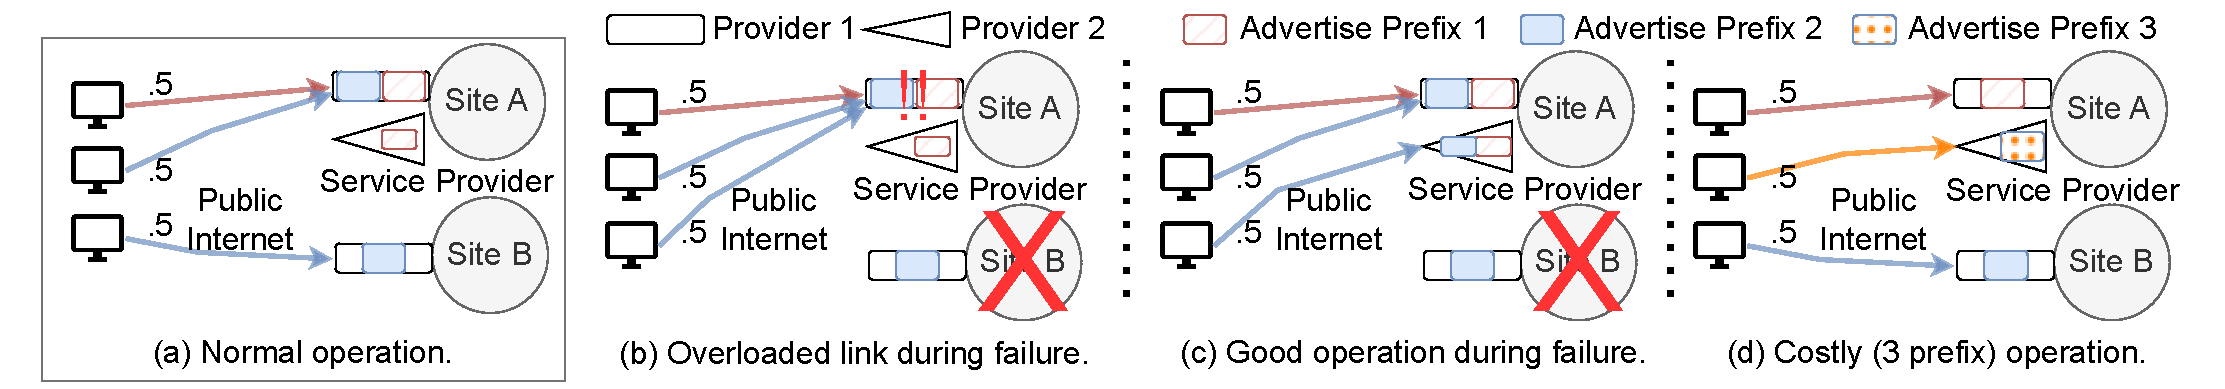
\includegraphics[width=.78\textwidth]{figures/motivating_resilience_example-all-in-one.drawio.pdf}
    \caption{The interdomain capacity-vs-latency dilemma.  (a)~Steady
        state: traffic is split between two sites by directing half
        of users to each prefix.  (b)~When site~B fails, BGP collapses
        all traffic onto Provider~1 at site~A, overloading the link
        even though global capacity is sufficient.
        (c)~\sparse's solution: advertise prefix~2 to Provider~2 at
        site~A \emph{before} the failure, so traffic can split across
        two providers when site~B goes down.
        (d)~The prohibitively expensive alternative: advertise one
        prefix per peering, which exceeds typical IPv4 prefix budgets
        by orders of magnitude.}
    \label{fig:mre}
\end{figure*}

\Cref{fig:mre} shows the core tension and previews \sparse's
solution.  Existing approaches address it in three ways, each with
a different failure mode.

\parab{Too specific.}  \fastroute, \anyopt, \painter,
and others~\cite{fastroute,calder2015analyzing,anyopt,regional-anycast,painter}
advertise different prefixes to subsets of peers, exposing more
paths to clients.  These systems optimise one objective at a time
--- typically steady-state latency.  They do not model capacity
explicitly, so a clever low-latency configuration can leave one
ingress carrying $69\%$ of post-failure traffic, as we measure for
\painter in \Cref{sec:eval-failure}.  Their objective-specific
greedy search also does not generalise: extending \painter to
optimise cost or resilience requires re-designing the search
strategy.

\parab{Too reactive.}  \tipsy~\cite{tipsy} drains links after they
overload by withdrawing advertisements.  This works only after the
overload is observed and re-converging BGP can take tens of seconds
to minutes, during which traffic suffers and configuration changes
may propagate undesirably
\cite{msft-bgp-outage,fb-bgp-outage,isp-bgp-outage}.

\parab{Too costly.}  \servprods often handle the problem by
overprovisioning capacity, but the overhead is substantial.  We
analysed 18~months of OVH per-link utilization data
\cite{ovh-weathermap} by splitting the data into successive 120-day
planning periods.  For each period we used the $95^{\mathrm{th}}$
percentile utilization of the previous period as the ``near-peak''
load, set the link's next-period capacity to that value times an
overprovisioning factor, and counted 5-minute intervals where
utilization exceeded $100\%$.  \Cref{fig:ovh_utilization} shows
the resulting trade-off across 41~OVH sites and 1{,}650~links:
a 30\% factor yields $60$--$70\%$ median utilization but
thousands of congestive events per period; eliminating most events
requires keeping median utilization around 50\%.  Because peering
capacity has fixed costs (fibre, line cards, CDN servers) and
variable costs (power, transit)
\cite{jupiter-evolving,facebook-capacity-planning,taiji,cascara},
this idle capacity is expensive.

\begin{figure}[t]
    \centering
    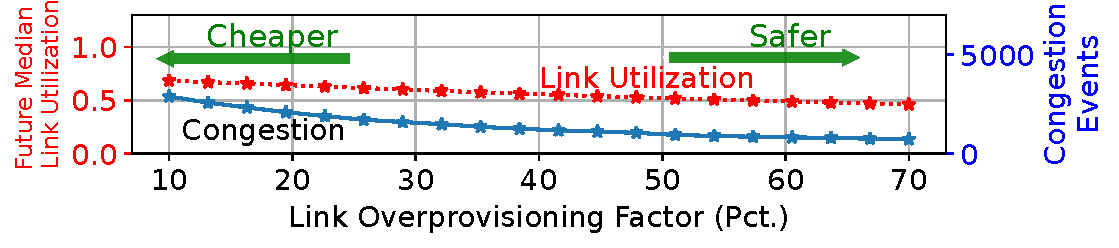
\includegraphics[width=.78\columnwidth]{figures/median_utilization_over_overprovisioning.pdf}
    \caption{To avoid congestive events on OVH's network, operators
        must overprovision so heavily that median link utilization
        falls below 50\%.}
    \label{fig:ovh_utilization}
\end{figure}

\subsection{What a better system needs}
\label{sec:motivation-what-we-need}

\Cref{fig:mre}c shows that there exists a configuration that
avoids overload at no extra prefix cost --- it just requires
finding the right one before failure happens.  This observation
motivates the design goals in \S\ref{sec:design}.  The challenge
is search: with a typical \servprod connected to ${>}10$\,k
peerings~\cite{cloudflare-peering-numbers}, the configuration space
exceeds~$2^{10{,}000}$.  Even one Internet measurement per
configuration would take centuries because BGP advertisements
must be spaced minutes apart to avoid route-flap dampening.
\sparse's job is to find good configurations using only tens to
hundreds of real measurements.

%==============================================================
\section{SCULPTOR Design}
\label{sec:design}

\subsection{Design goals}
\label{sec:design-goals}

We designed \sparse to meet five goals:

\parab{G1. Support arbitrary objective functions.}  A \servprod
should be able to express different goals (latency,
capacity, cost, traffic-class priorities, resilience to failures)
and combinations of them, without redesigning the solver.

\parab{G2. Be proactive.}  Decisions must be made before failures,
flash crowds, or other disruptive events, not in response to them
--- both to avoid the BGP-change risk and to escape the open-loop
delay of reactive systems.

\parab{G3. Scale to provider sizes.}  The solver must handle the
$>$10\,k peerings of a real public cloud, where the discrete
advertisement space exceeds $2^{10{,}000}$ and the traffic
allocation problem has $>$100\,M constraints
(\S\ref{sec:optimization-formulation}).

\parab{G4. Deploy unilaterally.}  A \servprod must be able to
deploy the system using only standard BGP.  No source-AS
coordination, no SCION-style buy-in, no proprietary peer features.

\parab{G5. Disruption-free.}  The solver's planning phase must not
move live production traffic.  Live traffic should follow new
routes only after the configuration has converged.

\subsection{Architecture overview}
\label{sec:design-overview}

\begin{figure}[t]
    \centering
    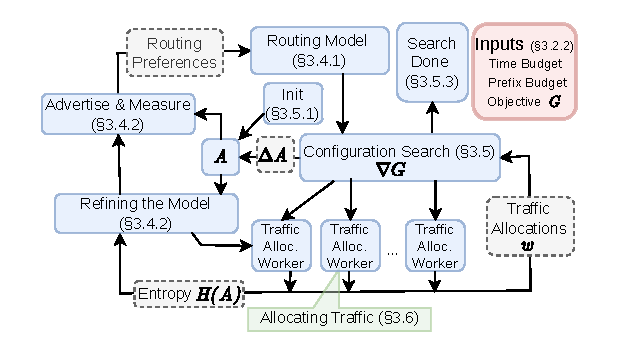
\includegraphics[width=.85\columnwidth]{figures/motivating_resilience_example-system diagram.drawio.pdf}
    \caption{\sparse's architecture.  The probabilistic routing
        model converts a small number of real BGP measurements
        into estimates of $G(R(A),w)$ for any candidate
        configuration~$A$.  The outer gradient-descent loop drives
        $A$ toward a minimum of~$G$, querying the model for objective
        and gradient values.  Each model query spawns inner-loop
        traffic-allocation problems that solve for the best~$w$
        given~$A$.  Exploration sends a small number of test
        advertisements per outer iteration to refine the model
        where its uncertainty is highest.}
    \label{fig:system_overview}
\end{figure}

\Cref{fig:system_overview} shows the three pieces of \sparse's
design:

\parab{Probabilistic routing model.}  We cannot measure the
routing function $R(A)$ directly --- doing so for every candidate
configuration would take centuries.  Instead, \sparse keeps a
distribution over which ingress each user group prefers, refines
it from a small number of real BGP advertisements, and exposes a
\emph{tractable} expectation of $G(R(A),w)$ as a function of the
continuous relaxation $\tilde A$.

\parab{Optimizer.}  The outer loop runs gradient descent on
$G$ over $\tilde A$.  Because $G$ also depends on the traffic
allocation~$w$, each outer step invokes an inner loop that solves
a linear program for the optimal $w$ given~$\tilde A$.  The
discrete configuration $A$ is recovered by thresholding $\tilde A$
at $0.5$.

\parab{Exploration.}  A handful of times per optimization run,
\sparse issues a real BGP advertisement to a configuration where
its model is most uncertain (highest Shannon entropy of the
predicted~$G$).  The resulting measurements update the model and
sharpen its predictions on all neighbouring configurations.

The key design decision is the split between a learned, black-box
routing model and a structured, gradient-friendly optimizer.  This
lets \sparse satisfy G1 (any differentiable~$G$ plugs in), G3
(both loops parallelise trivially), and G5 (only the handful of
exploration measurements touch real BGP).  The proactive nature of
the optimizer satisfies G2, and the BGP-only interface satisfies G4.

\subsection{How SCULPTOR differs from \painter and \anyopt}
\label{sec:design-differentiation}

\painter~\cite{painter} and \anyopt~\cite{anyopt} are the
closest prior systems.  Both pre-compute BGP advertisements to
improve steady-state latency for ingress traffic.  \sparse differs
in three ways that map directly to design goals:

\noindent\textbf{Multi-objective vs single-objective.}  \painter
greedily picks the prefix-peering pairs that most reduce average
latency; \anyopt randomly samples and keeps good ones.  Neither
search procedure makes sense for ``minimize cost subject to
capacity'' or ``minimize HP-class congestion'': capacity violation
penalties, multi-class trade-offs, and failure regularisers do not
plug into greedy or random search.  \sparse takes any
differentiable~$G$, including non-trivial penalties for over-utilisation
and resilience (\S\ref{sec:optimization-objectives}).

\noindent\textbf{Capacity awareness.}  \painter and \anyopt assume
each ingress has infinite capacity.  This makes their
configurations brittle: a small failure can move millions of clients
onto one link.  \sparse's objective penalises over-utilisation in
expectation, both in steady state and under modelled single-link
and single-site failures.

\noindent\textbf{Scale of search.}  \painter measures a few thousand
configurations during its greedy search; \anyopt measures the
samples it draws.  \sparse evaluates roughly $20$\,M configurations
per Internet measurement because gradient steps in the continuous
relaxation are cheap (they query the routing model, not BGP).
\Cref{sec:why-sparse-works} quantifies the impact on result quality.

%==============================================================
\section{Optimization}
\label{sec:optimization}

This section formalises the optimization problem
(\S\ref{sec:optimization-formulation}), names three concrete
objective functions that \sparse handles
(\S\ref{sec:optimization-objectives}), describes the probabilistic
routing model and how it learns from a few Internet measurements
(\S\ref{sec:optimization-model}--\S\ref{sec:optimization-exploration}),
and presents the two-loop solver
(\S\ref{sec:optimization-solver}).
\Cref{tab:term_definition} in \Cref{ap:notation} tabulates every
symbol used in this section.

\subsection{Problem formulation}
\label{sec:optimization-formulation}

\parab{Setting.}  A \servprod operates tens to hundreds of
geo-distributed sites~\cite{msft-wan-numbers}, each with a finite
serving capacity, and connects to other ASes via thousands of
peering links across those sites, each with a finite link capacity.
We group clients into \emph{user groups} (\ugs) --- sets of clients
that route similarly, e.g.\ /24 prefixes or metropolitan regions
--- and assume the \servprod knows or can measure each \ug's
traffic volume $v(\unenclug)$ and round-trip latency to each
ingress (a standard assumption supported by deployed measurement
systems
\cite{odin,end-user-mapping,verfploeter,calder-nel,anyopt,painter}).
We model paths as bottlenecked at the ingress link, in line with
recent Internet flattening
\cite{todd-cloud-connectivity}; handling violations of this
assumption (e.g.\ peering-network congestion) is exactly a
failure event, which \sparse explicitly models in
\S\ref{sec:optimization-objectives}.

\parab{Decision variables.}  An \emph{advertisement configuration}
$A$ is a binary vector with one entry per \peerprefix~pair: $A(p,l)=1$
iff prefix $p$ is advertised at peering link $l$.  The traffic
allocation $w$ is a non-negative real-valued vector with one entry
per $\langle p, \unenclug\rangle$ pair, where $w(p,\unenclug)$ is the
volume of \ug~$\unenclug$'s traffic sent toward prefix~$p$.
Implementing the configuration in BGP produces a \emph{routing
function} $R(A)$ that maps each $\langle p,\unenclug\rangle$ to the
ingress link on which traffic arrives at the \servprod.  We write
$e(R(A)(p,\unenclug))=1$ when a route exists for that pair and 0
otherwise.

\parab{General problem.}  Given an objective $G(R(A),w)$ (e.g.\
average latency, peak link utilisation, traffic cost, or a
weighted combination), we solve:
\begin{equation}
\label{eq:general_problem}
\begin{aligned}
\min_{A,w}\quad & G(R(A),w) \\
\textrm{s.t.}\quad
& w(p,\unenclug)\geq 0,\quad A(p,l)\in\{0,1\}\quad \forall \unenclug,p,l, \\
& \sum_{p} w(p,\unenclug)\, e(R(A)(p,\unenclug)) = v(\unenclug)\quad \forall \unenclug.
\end{aligned}
\end{equation}
The first constraint enforces variable types; the second requires
that every \ug's traffic is fully placed on \emph{some} working
route.  The optimization has tens of thousands of binary
configuration variables and millions of allocation variables, so
the problem is well beyond any off-the-shelf MILP solver at
provider scale (\S\ref{sec:implementation}); the bulk of
\S\ref{sec:optimization-solver} is about making it tractable.

\subsection{Three objective functions}
\label{sec:optimization-objectives}

We use \Cref{eq:general_problem} to instantiate three objectives;
the same framework supports others.

\parab{Latency under capacity constraints.}  The basic latency
objective is the traffic-weighted average ingress latency
$\mathcal{L}(\unenclug,l)$.  To penalise overload we add a
maximum-link-utilisation regulariser controlled by $\beta$:
\begin{equation}
\label{eq:mlu_constraint}
G_{\mathrm{lat}}(R(A),w) \;=\;
\frac{\sum_{\unenclug} v(\unenclug)\,\mathcal{L}(\unenclug, R(A))}
     {\sum_{\unenclug} v(\unenclug)}
\;+\; \beta\,M(A,w),
\end{equation}
where $M(A,w)$ is the maximum utilisation across links.

\parab{Resilience to unseen events.}  We harden $G_{\mathrm{lat}}$
by adding the average objective value over modelled single-link
and single-site failures: for each link~$l$ we define a binary
failure mask $F_l$ that zeros out the corresponding column of $A$,
and write
\begin{equation}
\label{eq:failure_reg}
G_{\mathrm{res}} \;=\; G_{\mathrm{lat}}(R(A),w)
     \;+\; \sum_{l\in\mathcal F}\alpha_l\,
       G_{\mathrm{lat}}\!\bigl(R(A\!\odot\! F_l), w_{F_l}\bigr).
\end{equation}
The $\alpha_l$ weight per-failure importance.  Configurations that
do well under \Cref{eq:failure_reg} have good primary \emph{and}
backup paths.  By the deep-learning intuition that ``training
under perturbations encourages wide minima''
\cite{huang2020understanding}, the failure regulariser also makes
\sparse robust to flash crowds and diurnal swings it never saw
during optimization (we confirm this experimentally in
\S\ref{sec:eval-efficiency}).

\parab{Multi-class priorities.}  Following private-WAN TE practice
\cite{swan,b4} we split traffic into high- and low-priority classes
and minimise the weighted sum of HP average latency and HP
congested traffic, with a cap on per-link total utilisation so the
low-priority class cannot collapse onto one link.

\parab{Per-site cost.}  Each site $s$ has a cost-per-byte $c_s$
(modelling, e.g., per-region power price or carbon intensity).
We add $\lambda\sum_s c_s\,(\text{volume at }s)$ to
$G_{\mathrm{lat}}$.

In all three objectives, the dependence on $R(A)$ is what makes
\Cref{eq:general_problem} hard --- $R$ is a discontinuous,
hard-to-sample function of $A$.  The next two subsections describe
how \sparse approximates it.

\subsection{Probabilistic routing model}
\label{sec:optimization-model}

\sparse maintains a probability distribution over $R(A)$ rather
than a single best estimate, because interdomain routing decisions
depend on hidden BGP policies that are difficult to infer
directly~\cite{sermpezis2019inferring,tipsy}.  A priori, every
ingress at which a
prefix is advertised is equally likely to be the one each \ug
uses for that prefix, provided the \ug has any route through that
ingress (the \servprod can determine reachability cheaply from
existing measurements
\cite{odin,end-user-mapping,verfploeter,calder-nel}).

\begin{figure}[t]
    \centering
    \begin{subfigure}{.47\columnwidth}
        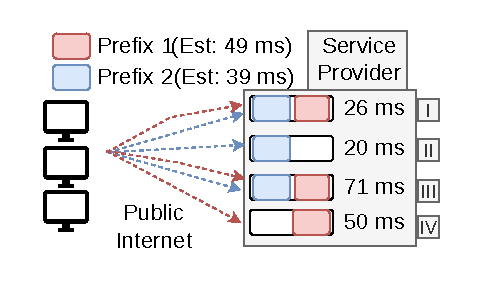
\includegraphics[width=\columnwidth]{figures/explaining_methodology-apriori.drawio.pdf}
        \caption{Before any measurement.}
        \label{fig:learning_description_pre}
    \end{subfigure}\hspace{.02\columnwidth}
    \begin{subfigure}{.47\columnwidth}
        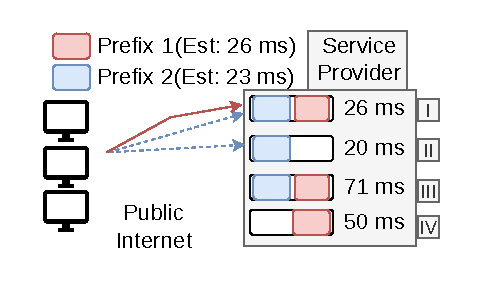
\includegraphics[width=\columnwidth]{figures/explaining_methodology-post.drawio.pdf}
        \caption{After advertising the red prefix.}
        \label{fig:learning_description_post}
    \end{subfigure}
    \caption{Refining the routing model.  A \ug can reach two
        prefixes (red, blue) via several ingresses.  Initially
        each ingress is equally likely (a), so \sparse estimates
        the \ug's latency to each prefix as the average over
        ingresses.  After advertising the red prefix and observing
        that ingress~1 is preferred over ingresses~3 and~4, \sparse
        rules those ingresses out for the blue prefix too (b),
        producing a sharper estimate of the latency to the blue
        prefix \emph{without advertising it}.}
    \label{fig:learning_distributions}
\end{figure}

\sparse refines the distribution by issuing test advertisements.
When a \ug is observed to take one ingress over another for some
prefix, \sparse permanently rules out the less-preferred ingress
for that \ug across \emph{all} prefixes for which both ingresses
are an option.  This single observation propagates: the latency
estimate to a prefix the \ug has never seen advertised tightens
because some of its hypothetical ingresses are now known to be
non-preferred (\Cref{fig:learning_distributions}).

Many objectives of interest are robust to imperfect knowledge of
$R(A)$.  Most \ugs reach a given \servprod \emph{site} with similar
latency over its various ingresses~\cite{brandon-facebook-imc};
predicting the right site is usually sufficient to predict the
latency, even if the exact ingress is uncertain.  This is why a
distribution suffices --- we only need the expectation of $G$, not
a point estimate of $R$.

\begin{figure}[t]
    \centering
    \begin{subfigure}{.47\columnwidth}
        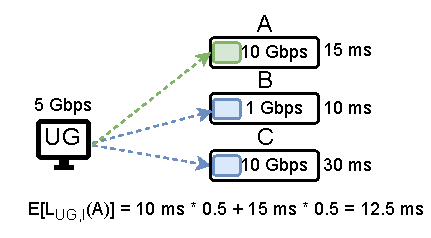
\includegraphics[width=\columnwidth]{figures/explaining_methodology-user_probability.drawio.pdf}
        \caption{Without capacity.}
        \label{fig:user_probability}
    \end{subfigure}\hspace{.02\columnwidth}
    \begin{subfigure}{.47\columnwidth}
        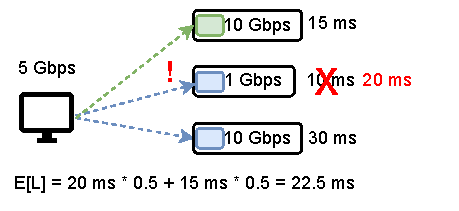
\includegraphics[width=\columnwidth]{figures/explaining_methodology-user_probability_3.drawio.pdf}
        \caption{With capacity penalty.}
        \label{fig:user_probability_3}
    \end{subfigure}
    \caption{Capacity-aware expectation.  The green prefix is
        advertised only via ingress~A; the blue prefix is advertised
        via ingresses~B and~C, each equally likely.  In~(a) the
        \ug's expected latency averages over both blue options.
        In~(b) ingress~B is over-capacity with 50\% probability;
        \sparse inflates the latency contribution from ingress~B
        accordingly, discouraging configurations that crowd a link.}
    \label{fig:modeling_latency_description}
\end{figure}

\parab{Capacity-aware expectation.}  For objectives that include a
capacity penalty (\Cref{eq:mlu_constraint}), \sparse first computes
the distribution of \ug-to-ingress assignments, then computes the
distribution of link utilisations, and then inflates the latency
contribution of any \ug whose chosen ingress is over-capacity in
expectation (\Cref{fig:modeling_latency_description}).  This
penalty is a one-shot heuristic --- we do not re-route \ugs after
inflating their latencies, which would create an infinite loop ---
but it pushes the optimizer away from concentrated solutions.

\subsection{Exploration via Shannon entropy}
\label{sec:optimization-exploration}

The routing model is only useful if it learns the right things.
Per outer-loop iteration, \sparse identifies up to a handful of
\emph{adjacent} configurations --- those differing from the
current $A$ by a single advertisement, or those corresponding to a
single failure $A \odot F_l$ --- and picks the one whose
\emph{distribution of $G$} has the highest Shannon entropy under
the current model.  It advertises that configuration on the
Internet, observes the resulting routes, and updates the model.
Targeted exploration converges substantially faster than the
greedy~\cite{painter} or random~\cite{anyopt} alternatives
(\S\ref{sec:why-sparse-works}, \Cref{fig:uncertainty_path_measures_over_iterations}).

\subsection{Two-loop solver}
\label{sec:optimization-solver}

Even with the model, \Cref{eq:general_problem} is a discrete,
non-convex, multi-million-variable problem.  We split it into an
outer loop over configurations (gradient descent) and an inner
loop over traffic allocations (an off-the-shelf LP solver).

\parab{Outer loop: gradient descent on a continuous relaxation.}
We introduce $\tilde A \in [0,1]^{|A|}$, treat
$G(R(\tilde A), w)$ as the model's expectation evaluated at
\emph{integer} corners of $\tilde A$, and interpolate between
corners with sigmoids~\cite{langer2021approximating}.  Gradients
are computed coordinate-wise; we subsample and keep the largest
gradient entries to amortise work over millions of dimensions
\cite{shechtman2014gespar}.  At the end of optimization we
threshold $\tilde A$ at $0.5$ to recover the discrete configuration~$A$.
Gradient descent converges to a local minimum for bounded
objectives~\cite{li2024convex}; we evaluate empirical convergence
in \S\ref{sec:evaluation}.

\parab{Inner loop: traffic allocation.}  For each outer-loop
gradient evaluation, \sparse needs the optimal $w$ for the
configuration under consideration.  Given $R(A)$, all three
objectives in \S\ref{sec:optimization-objectives} are linear in
$w$, so off-the-shelf LP solvers find the global optimum.  Other
non-convex objectives sometimes have efficient
heuristics~\cite{cascara}, which plug into the inner loop without
changing anything else.

\parab{Scaling.}  Outer-loop work is dominated by the product of
prefix budget and ingress count and is embarrassingly parallel.
Inner-loop work scales with the number of Monte-Carlo samples used
to evaluate the expectation; we provide an exact closed-form
analogue for the latency objective in \Cref{ap:heuristics} that
yields a $50\times$ speedup at a $2$\,ms average-latency cost.

\parab{Bottleneck.}  In practice, the wall-clock bottleneck is the
20-minute inter-advertisement delay that \sparse leaves between
exploration steps to avoid route-flap dampening.  Gradient descent
\emph{between} advertisements is cheap.

%==============================================================
\section{Implementation \& Evaluation Setup}
\label{sec:implementation}

We implement \sparse in ${\sim}7$\,k lines of Python (gradient
descent with Nesterov acceleration~\cite{nesterov2018lectures};
Gurobi~\cite{gurobi} for inner-loop LPs; learning rate $0.01$ with
decay, $\alpha_l=4.0$).  We evaluate it both on the public
Internet via PEERING on Vultr and in an emulator that lets us
sweep deployment sizes.

\subsection{Vultr + PEERING prototype}

\sparse advertises BGP prefixes via the
PEERING~\cite{schlinker19peering} testbed, now deployed at
32~Vultr cloud sites~\cite{vultr}.  Vultr peers with
${>}10$\,k networks, giving \sparse access to a realistic
provider-scale routing surface.

\parab{Client measurements.}  We probe each /24 to find 5\,M
responsive IPv4 targets.  Using Vultr's advertised reachability,
we identify direct-peer routes (excluding route-server peers
\cite{chatzis2013there}) and measure per-\ug latency to each
peer by advertising a prefix via that peer alone using Vultr's
BGP communities and pinging clients from a Vultr VM.  Removing
addresses whose minimum RTT is ${<}1$\,ms (likely infrastructure)
leaves 666\,k /24s with paths through 825~Vultr ingresses.

\parab{Internet experiments.}  We use RIPE Atlas
probes~\cite{ripe-atlas} to measure paths to prefixes we announce
from PEERING, limited to 10~major-hub sites to stay within RIPE
Atlas's 15\,k traceroutes/day budget.  This yields 972 networks
across 38~countries, each with roughly 60 candidate ingresses; we
use 12 prefixes and at most one advertisement per hour.

\parab{Emulator.}  To scale beyond the RIPE Atlas budget, we
emulate routing using the measured latencies and a learned
preference model.  We sweep deployment sizes
$\{3,5,10,15,20,25,32\}$ sites and run 10~random subsets of
\ugs, demands, and preferences per size.  Across all emulator
runs we cover 52\,k client prefixes (31\% of APNIC population)
and 873~ingresses.  Prefix budget is one tenth of ingress count
(10 prefixes for 3 sites, up to 60 for 32 sites), consistent with
prior practice~\cite{anyopt,painter}.

\subsection{Traffic volumes and capacity}

We model \ug volumes two ways: \emph{random} (per-site total
in $[1,10]$, divided among the \ugs that anycast routes to the
site, within one order of magnitude) and \emph{APNIC-populated}
(volumes proportional to APNIC AS populations
\cite{apnic_pop_est,loqman-apnic}).  High-level results are
qualitatively identical, so we report the random version below.

For capacity, we provision each link to $30\%$ above its
near-peak load under anycast, the lower end of the OVH-derived
range in \Cref{fig:ovh_utilization}.  Sites get $30\%$ above their
anycast-aggregate load.  Because we are not the \servprod and
cannot directly measure ingress assignment, we use BGP-announced
prefix routes from RIPE Atlas traceroutes for the Internet
experiments and our emulator's learned preferences for the
emulator runs.

\subsection{Baselines}

We compare \sparse against:
\acast (single prefix advertised to all peers, the standard
availability baseline);
\ucast (one unique prefix per site);
\painter~\cite{painter} (state-of-the-art proactive latency-only system);
\anyopt~\cite{anyopt} (random-sampling latency optimizer); and
\expensive (one prefix per peering --- not realisable because of
prefix cost, but it is the relevant optimum because any restriction
on prefix budget is a special case).  We report differences against
\expensive throughout so the gap to the unrealisable optimum is
always visible.

%==============================================================
\section{Evaluation}
\label{sec:evaluation}

We answer five questions:
\begin{description}
\item[Q1] How close does \sparse get to the unrealisable
          per-peering optimum on steady-state latency, on both
          the public Internet and in emulation?
          (\S\ref{sec:eval-steady-state})
\item[Q2] Does \sparse maintain that lead under \emph{unseen}
          conditions --- single-link failures, single-site
          failures, flash crowds, and diurnal swings?
          (\S\ref{sec:eval-failure}--\S\ref{sec:eval-efficiency})
\item[Q3] Can \sparse satisfy multiple traffic classes
          simultaneously? (\S\ref{sec:eval-multiple-traffic-classes})
\item[Q4] Can \sparse trade off latency against per-site cost?
          (\S\ref{sec:eval-per-site-costs})
\item[Q5] What in \sparse's design produces these gains?
          (\S\ref{sec:why-sparse-works})
\end{description}

We summarise the headline findings:
\begin{itemize}
\item \sparse comes within $2.0$\,ms of the per-peering optimum
      on the Internet, vs $5.5$\,ms for \painter.
\item Under single-site failures \sparse uncongests
      $98.4\%$ of traffic; \painter overloads $69.6\%$.
\item On 32-site emulated deployments, \sparse absorbs a
      $3\times$ flash crowd before any link congests --- $26\%$
      more headroom than \painter.
\item For multi-class priorities \sparse halves the congestion
      experienced by high-priority traffic compared to \painter
      and \ucast.
\item For per-site cost, \sparse's objective gap to \expensive is
      $1.5$--$3\times$ smaller than \painter's.
\end{itemize}

\subsection{Q1: Steady-state latency}
\label{sec:eval-steady-state}

\begin{figure*}[t]
    \centering
    \begin{subfigure}{.32\textwidth}
        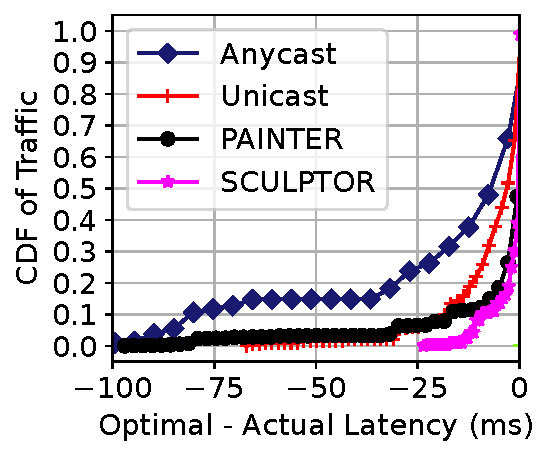
\includegraphics[width=\columnwidth]{figures/steady_state_latency_actual_deployment.pdf}
        \caption{Internet (CDF of gap to \expensive).}
        \label{fig:steady_state_latency_actual_deployment}
    \end{subfigure}~
    \begin{subfigure}{.32\textwidth}
        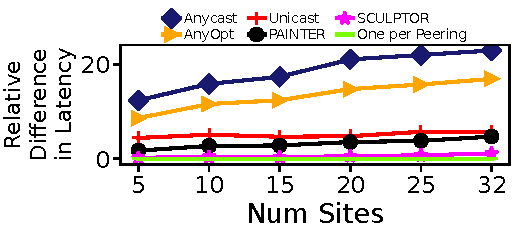
\includegraphics[width=\columnwidth]{figures/average_latency_over_deployment_size_normal.pdf}
        \caption{Emulator (average gap by size).}
        \label{fig:average_normal_over_dpsize}
    \end{subfigure}~
    \begin{subfigure}{.32\textwidth}
        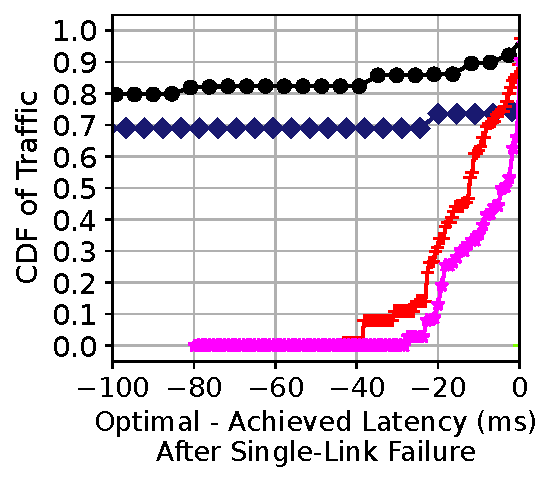
\includegraphics[width=\columnwidth]{figures/link_failure_latency_actual_deployment.pdf}
        \caption{Internet, link failure.}
        \label{fig:link_failure_latency_actual_deployment}
    \end{subfigure}
    \caption{Steady-state and failure latency.  \sparse stays
        closest to the unrealisable \expensive optimum across both
        the Internet deployment and emulated deployments of all
        sizes; the gap to \painter widens under failures.}
    \label{fig:latency_results}
\end{figure*}

\parab{Internet.}
\Cref{fig:steady_state_latency_actual_deployment} shows the
traffic-weighted CDF of the gap between each system's per-\ug
latency and \expensive's.  \sparse is on average $2.0$\,ms above
the optimum; \painter is $5.5$\,ms; \ucast and \acast are worse
still.  \sparse serves $91.8\%$ of traffic within $10$\,ms of
optimum, against $88\%$ for \painter.

\parab{Emulator.}
\Cref{fig:average_normal_over_dpsize} shows the same comparison as
deployment size grows.  \sparse's average gap to \expensive ranges
$0.1$--$2.4$\,ms across sizes; \painter is $1.1$--$2.2$\,ms worse
than \sparse, and \anyopt and \ucast do worse than both.
Aggregated across sizes, \sparse keeps $94.9\%$ of traffic within
$10$\,ms of \expensive, $99.2\%$ within $50$\,ms, and $99.9\%$
within $100$\,ms; \painter achieves $92.3\%$, $97.7\%$, and
$99.2\%$ respectively.

\subsection{Q2a: Single-link and single-site failures}
\label{sec:eval-failure}

We fail each ingress (or site) once, re-solve traffic
allocations, and re-measure latency for the \ugs that used the
failed element in steady state.  Traffic landing on an overloaded
link is excluded from the latency computation and reported
separately.

\parab{Internet, single-link failure.}
\Cref{fig:link_failure_latency_actual_deployment} shows \sparse
beats every other system on post-failure latency: its average
$7.9$\,ms gap to \expensive compares to $14.2$\,ms for \ucast
and substantially worse for the rest.  \painter loses control
entirely, overloading $69.6\%$ of post-failure traffic because
its capacity-blind search concentrated the failed link's load
onto one backup.

\parab{Internet, single-site failure.}  Trends repeat: \sparse
is $13.1$\,ms above optimum on average, the next-best system
(\ucast) is $25.1$\,ms above, and \painter overloads $95\%$ of
post-failure traffic.

\parab{Emulator.}  Across all deployment sizes,
\Cref{fig:50ms_link_failure_over_dpsize} shows \sparse keeps
$\geq 78.9\%$ of traffic within $10$\,ms of \expensive during
link failure, vs $66.1\%$ for \painter; under site failures
(\Cref{fig:50ms_site_failure_over_dpsize})
\sparse averages $8.7$\,ms above optimum with $18.5\%$ of traffic
overloaded, versus \painter's $14.7$\,ms and $34.8\%$.

\subsection{Q2b: Flash crowds and diurnal swings}
\label{sec:eval-efficiency}

A \emph{flash crowd} is a transient regional traffic surge
(content release, DDoS, breaking news).  We assign each client a
``home region'' based on its lowest-latency site, scale every
client's volume in one region at a time by $M\%$, recompute the
allocation, and find the lowest $M$ that overloads any link.

\Cref{fig:infrastructure_utilization_flash_crowd} shows the
critical $M$ averaged across regions.  At 32 sites \sparse
absorbs $\approx 3\times$ flash-crowd volume (vs roughly
$2.4\times$ for \painter), translating into a $3\times$ saving
versus the \acast-driven provisioning baseline and $26\%$ more
headroom than \painter.

We sample a diurnal traffic pattern from
\cite{taiji} (shape shown in \Cref{fig:diurnal_shape}) and
group sites by timezone, scaling peak-timezone
volume by $M\times$ and trough-timezone by $0.1M\times$.
\Cref{fig:infrastructure_utilization_diurnal} shows \sparse
sustains $24\%$ larger diurnal swings than \painter and
\ucast at 32 sites.  Both results follow from \sparse's
failure-regularised objective
(\Cref{eq:failure_reg}): planning for single-element failures
also produces routes that survive correlated regional load
spikes, even though \sparse never sees those patterns during
training.

\begin{figure}[t]
    \centering
    \begin{subfigure}{.48\columnwidth}
        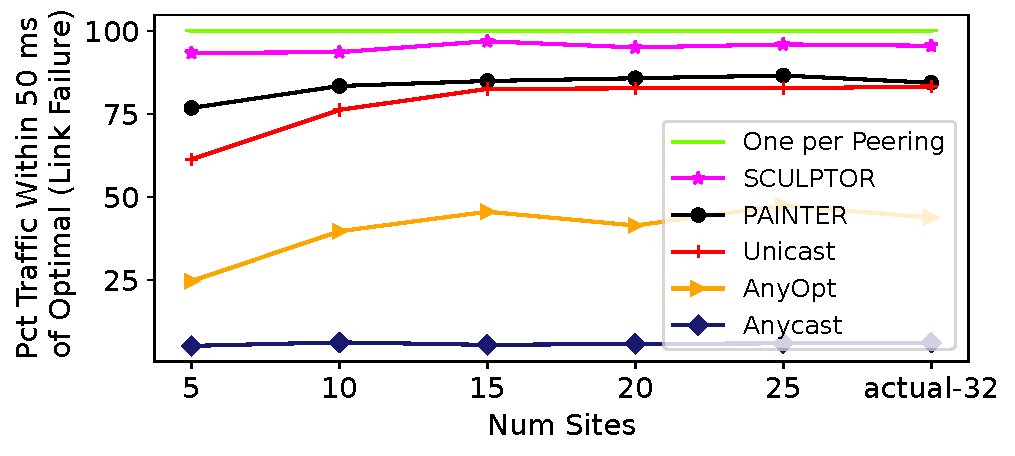
\includegraphics[width=\columnwidth]{figures/percent_traffic_within_50_ms_link_failure_over_deployment_size.pdf}
        \caption{\% traffic within 50\,ms of \expensive under link failure.}
        \label{fig:50ms_link_failure_over_dpsize}
    \end{subfigure}\hspace{.02\columnwidth}
    \begin{subfigure}{.48\columnwidth}
        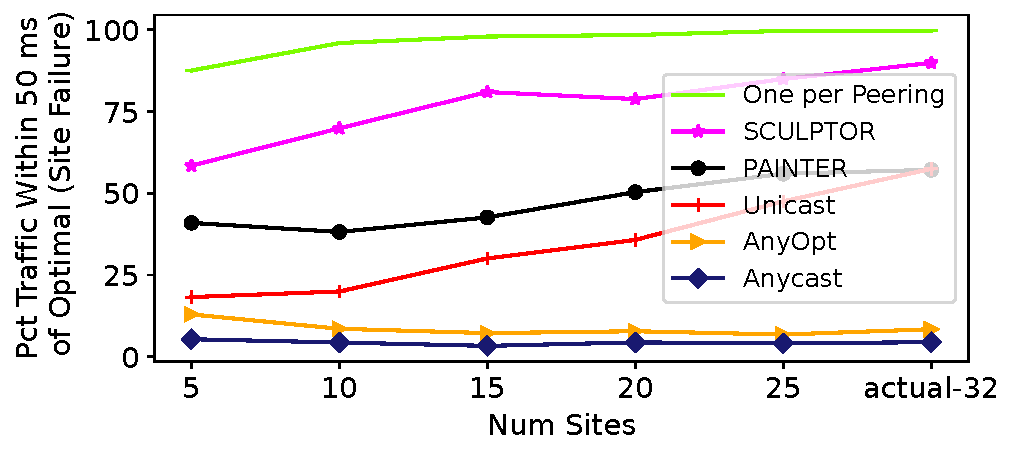
\includegraphics[width=\columnwidth]{figures/percent_traffic_within_50_ms_site_failure_over_deployment_size.pdf}
        \caption{\% traffic within 50\,ms of \expensive under site failure.}
        \label{fig:50ms_site_failure_over_dpsize}
    \end{subfigure}\\[.5em]
    \begin{subfigure}{.48\columnwidth}
        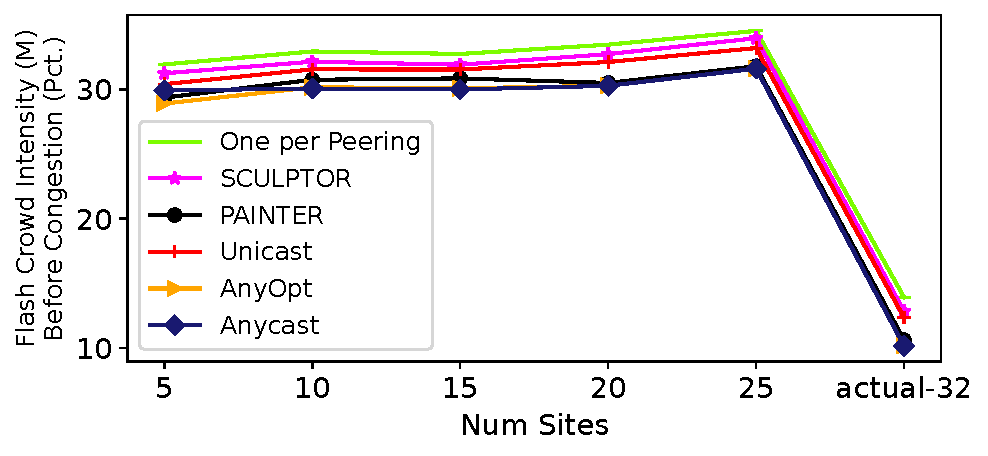
\includegraphics[width=\columnwidth]{figures/flash_crowd_blowup_before_congestion_over_deployment_size.pdf}
        \caption{Flash-crowd headroom.}
        \label{fig:infrastructure_utilization_flash_crowd}
    \end{subfigure}\hspace{.02\columnwidth}
    \begin{subfigure}{.48\columnwidth}
        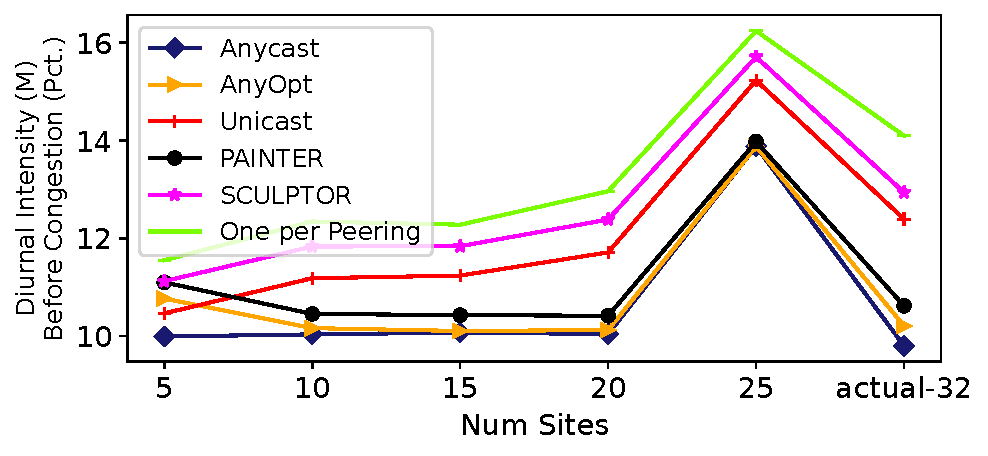
\includegraphics[width=\columnwidth]{figures/diurnal_blowup_before_congestion_over_deployment_size.pdf}
        \caption{Diurnal swing headroom.}
        \label{fig:infrastructure_utilization_diurnal}
    \end{subfigure}
    \caption{Resilience to unseen conditions.  \sparse maintains
        the largest fraction of traffic within 50\,ms of
        \expensive during failures and offers the most
        flash-crowd / diurnal headroom.  Failure-regularised
        training also generalises to unmodelled patterns.}
    \label{fig:single_element_failure}
\end{figure}

\subsection{Q3: Multiple traffic classes}
\label{sec:eval-multiple-traffic-classes}

We split traffic into high-priority (HP, latency-sensitive) and
low-priority (LP, bulk) and minimise the weighted sum of HP
average latency and HP congested traffic, with a per-link cap of
$10\times$ to keep LP from collapsing onto one link.  Links are
provisioned to $5\times$ HP volume, matching the LP/HP ratio
inferred from SWAN and B4~\cite{swan,b4}.

\begin{figure}[t]
    \centering
    \begin{subfigure}{.48\columnwidth}
        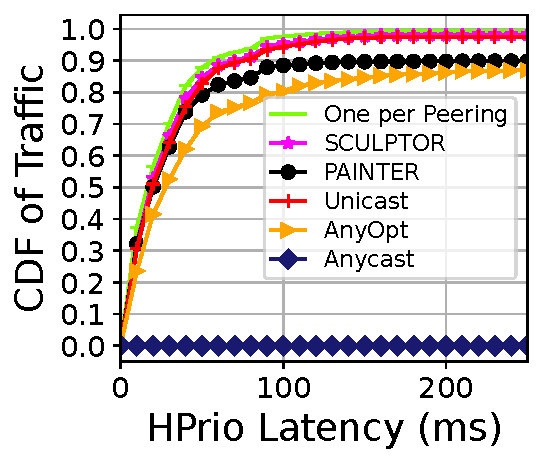
\includegraphics[width=\columnwidth]{figures/priority_bulk_traffic_latency.pdf}
        \caption{HP latency vs LP/HP ratio.}
        \label{fig:priority_bulk_traffic_latency}
    \end{subfigure}\hspace{.02\columnwidth}
    \begin{subfigure}{.48\columnwidth}
        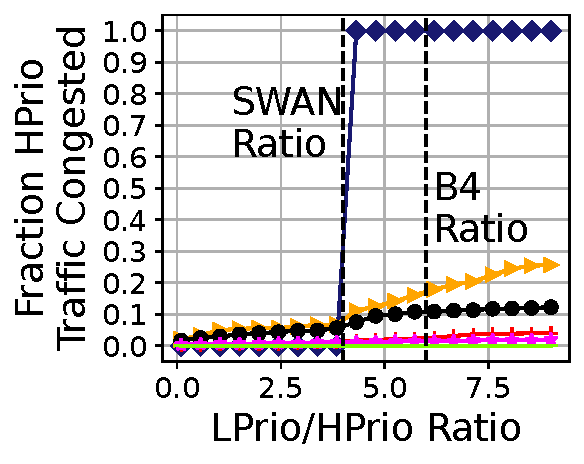
\includegraphics[width=\columnwidth]{figures/priority_bulk_traffic_congestion.pdf}
        \caption{HP congestion vs LP/HP ratio.}
        \label{fig:priority_bulk_traffic_congestion}
    \end{subfigure}
    \caption{\sparse routes high-priority traffic with lower latency
        and protects it from low-priority congestion better than
        every baseline.  We infer LP/HP ratios for SWAN~\cite{swan}
        and B4~\cite{b4} from those papers.}
    \label{fig:priority_bulk_traffic}
\end{figure}

\Cref{fig:priority_bulk_traffic_congestion} sweeps LP/HP ratio
from~0 to~5.  At ratio~$5$, \sparse achieves half the HP
congestion of \painter and \ucast; the
$\acast$ baseline becomes congested past ratio~$4$ because
global capacity runs out.  \Cref{fig:priority_bulk_traffic_latency}
shows \sparse also delivers HP latency closer to optimal than
every baseline at LP/HP~$=4$.  Capacity-aware planning matters:
\painter's latency-only objective is happy to put HP traffic on
the lowest-latency link even when that link is already crowded by LP.

\subsection{Q4: Per-site traffic cost}
\label{sec:eval-per-site-costs}

We assign each site a per-byte cost and minimise a weighted sum
of average latency and total cost.  We try three cost models:
random per-site costs, a step model where half the sites cost
$1.2\times$ the other half, and a carbon-intensity model based on
per-region $\mathrm{CO}_2$/kWh
\cite{electricity-carbon-data,carbon-intelligent-cdn}.

In all three, \sparse's objective gap to \expensive is the
smallest: under the step model, $1.5\times$ smaller than
\painter; under the carbon-intensity model, $3\times$ smaller.
When we increase the cost weight $100\times$, \sparse trades
$24$\,ms of average latency for $12\%$ lower per-site cost; its
objective gap to \expensive is $8\times$ smaller than \painter's
in this regime.  This confirms that \sparse can be tuned for
changing operator preferences without re-engineering the solver.

\subsection{Q5: Why \sparse works}
\label{sec:why-sparse-works}

\begin{figure}[t]
    \centering
    \begin{subfigure}{.48\columnwidth}
        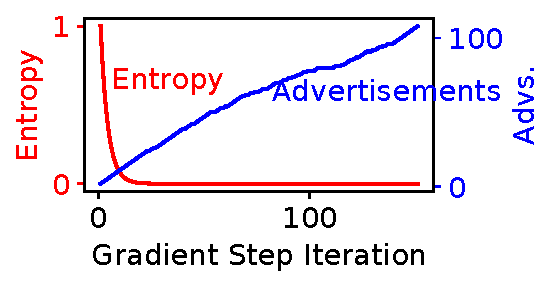
\includegraphics[width=\columnwidth]{figures/uncertainty_path_measures_over_iterations.pdf}
        \caption{Model entropy vs measurements.}
        \label{fig:uncertainty_path_measures_over_iterations}
    \end{subfigure}\hspace{.02\columnwidth}
    \begin{subfigure}{.48\columnwidth}
        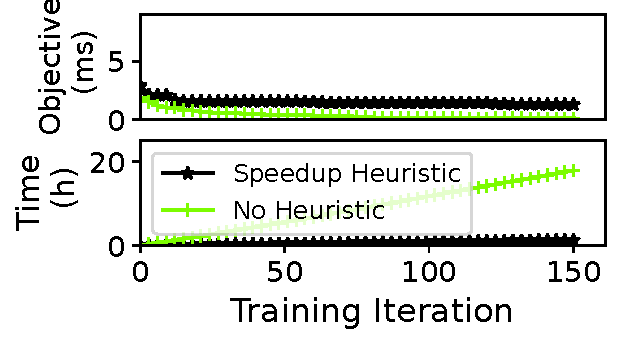
\includegraphics[width=\columnwidth]{figures/objective_heuristic_comparison_actual-10.pdf}
        \caption{Heuristic speedup vs accuracy.}
        \label{fig:heuristic_speedup}
    \end{subfigure}
    \caption{\sparse's model entropy decays exponentially with
        Internet measurements, so it stops needing them after
        a few tens.  The closed-form latency heuristic
        (\Cref{ap:heuristics}) gives a $50\times$ speedup at a
        $2$\,ms average-latency cost.}
    \label{fig:why-sparse-works}
\end{figure}

Three properties of \sparse's design produce these results.

\parab{It explores far more configurations than baselines.}  On a
32-site deployment, \sparse evaluates roughly $20$\,M configurations
across $200$ gradient steps; \painter measures
$\approx 2$\,k configurations; \anyopt samples $\approx 1$\,k.
The gap is a consequence of architecture: \sparse's gradient steps
query the routing model (cheap), not BGP (slow), so the inner
search is decoupled from the rate-limited measurement loop.

\parab{It measures where it is most uncertain.}
\Cref{fig:uncertainty_path_measures_over_iterations} shows the
maximum Shannon entropy of $G$ across unmeasured configurations
on the Internet deployment.  It decays exponentially: a small
number of entropy-targeted measurements suffices to make the
model confident across the whole search space, because each
preference observation rules out ingresses for \emph{many}
\ug-prefix combinations at once
(\S\ref{sec:optimization-model}).

\parab{It parallelises and admits heuristics.}  Both the outer
gradient computation and the inner-loop LP solves are
embarrassingly parallel across configurations and \ugs.
Latency-style objectives also admit a closed-form expectation
\Cref{ap:heuristics} that lets us replace Monte-Carlo sampling
with an exact analytic computation; in
\Cref{fig:heuristic_speedup} this delivers a $50\times$
inner-loop speedup at a $2$\,ms average-latency cost.

%==============================================================
\section{Related Work}
\label{sec:related}

\parab{Ingress traffic engineering.}  The systems closest to
\sparse are \painter~\cite{painter} and \anyopt~\cite{anyopt},
which we have discussed throughout.  \fastroute~\cite{fastroute}
load-balances anycast rings reactively; \tipsy~\cite{tipsy} drains
overloaded links by withdrawing routes; regional
anycast~\cite{regional-anycast,jiangchen-cdn-imc,tom-anycast,calder2015analyzing,end-user-mapping,cartographer,whyhigh,footprint-microsoft}
combines anycast and unicast at site granularity but does not
optimise advertisements globally.

\parab{Egress traffic engineering.}  Systems such as Espresso,
EdgeFabric, and Fastly's egress
TE~\cite{espresso,edge-fabric,fastly-egress} pick egress paths
from a \servprod to users; they sit on the other side of the
traffic flow and are complementary to \sparse.  Cost-aware egress
systems~\cite{entact,cascara,taiji} reshape traffic across egress
links to lower transit cost; \sparse adapts that idea for
\emph{ingress} using the public Internet rather than a private
backbone.

\parab{Intradomain failure planning.}  Private-WAN systems
\cite{hose-benders-facebook,evolve-or-die,blast-shield,google-capa-nsdi,r3,ffc,lancet,pcf}
plan intra-domain routes to survive $k$-component failures;
\sparse solves a different problem (interdomain, with limited
visibility into possible paths and capacities) and complements
these systems by helping a \servprod shift traffic away from
failed regions while preserving performance.

\parab{Cross-domain overlays.}  OTTER~\cite{otter-nsdi25}
orchestrates a multi-WAN overlay between a 5G operator and a
cloud, with on-demand flow placement.  \sparse and OTTER target
adjacent problems: OTTER engineers paths \emph{between} two
collaborating WANs through cloud-native overlays, while \sparse
engineers ingress paths from the global Internet using only BGP.
SCION~\cite{scion_deployment_conext} provides path control at the inter-AS layer
but requires ISP deployment.

%==============================================================
\section{Discussion \& Conclusion}
\label{sec:discussion-conclusion}

Decades of intradomain traffic-engineering progress have rested on
unilateral, programmable network primitives --- fast
reroute~\cite{frr-rfc}, virtual routing and
forwarding~\cite{vrf-rfc}, virtual output queueing~\cite{voq-info}.
Interdomain proposals that need cross-AS coordination
(IntServ/DiffServ~\cite{diffserv-rfc},
L4S~\cite{l4s-rfc}, MIRO~\cite{miro}) have seen little deployment.
\sparse stays inside the unilateral envelope: it uses only BGP and
deploys without coordination, yet it gives \servprods a single
solver that can target latency, capacity, cost, and resilience at
provider scale.

\sparse is a starting point, not a finished story.  We see three
threads worth picking up.  First, richer BGP configurations ---
community tags, traffic-class signalling --- would enrich the
configuration space and likely tighten the gap to \expensive.
Second, \sparse's failure regulariser is currently single-element;
correlated failures (whole regions, shared infrastructure)
deserve their own treatment.  Third, integrating \sparse with
overlay systems such as OTTER~\cite{otter-nsdi25} could let a
\servprod span both the public Internet and partner WANs with
one optimisation framework.

We conclude that black-box, gradient-based optimisation is the
right approach for multi-objective interdomain ingress traffic
engineering, and that the rapid empirical convergence of \sparse's
routing model (\Cref{fig:uncertainty_path_measures_over_iterations})
makes the approach practical at provider scale.
\label{sec:end-of-conclusion}

%==============================================================
\paragraph*{Ethics statement}
This work raises no human-subjects concerns.  All routing
experiments use prefixes allocated to the PEERING testbed
\cite{schlinker19peering}, an academic-research facility with an
IRB-style review process for new experiments, and all measurements
involve BGP advertisements toward experimenter-controlled prefixes
plus active probes from researcher-operated VMs to public IP
addresses.  No production traffic of Vultr or any third party was
diverted or affected.  Our latency measurements record per-/24
round-trip times and contain no payload, no port-level
information, and no PII.  The OVH utilisation
dataset~\cite{ovh-weathermap} is publicly published by OVH;
the APNIC population dataset~\cite{apnic_pop_est} is publicly
published by APNIC.  Our open-source artefact is anonymised for
double-blind review and will be released under a permissive
licence on acceptance.

\paragraph*{Generative AI disclosure}
The authors used a GenAI-based coding assistant during paper
preparation for prose editing and
LaTeX formatting. The assistant did not generate experimental
results, claims, numerical findings; all
results in this paper were produced by the authors' implementation
and verified by the authors.

%==============================================================
\bibliography{mybib}

\appendix

%==============================================================
\section{Notation}
\label{ap:notation}

\Cref{tab:term_definition} lists every symbol used in
\S\ref{sec:optimization}, for reference while reading the body.

\begin{table}[h]
\caption{Notation used in the optimization formulation
         (\S\ref{sec:optimization}).}
\label{tab:term_definition}
\centering
\small
\begin{tabular}{|ll|}
\hline
\multicolumn{2}{|c|}{\textbf{Variables}} \\ \hline
$A$              & advertisement configuration over peers and prefixes \\ \hline
$w$              & traffic allocation to routes (non-negative real) \\ \hline
$R$              & routing function, maps configurations to ingress assignments \\ \hline
$p$              & prefix, one of many in a (limited) prefix budget \\ \hline
$l$              & ingress link, \servprods often have thousands \\ \hline
$c(l)$           & capacity of link $l$ \\ \hline
$\unenclug$      & user group (e.g.\ a /24 or a metropolitan area) \\ \hline
$w(p,\unenclug)$ & traffic from \unenclug{} directed to prefix $p$ \\ \hline
$G$              & objective function (e.g.\ average latency, peak utilization) \\ \hline
$v(\unenclug)$   & steady-state traffic volume of \unenclug \\ \hline
$F_l$            & failure mask for link $l$ \\ \hline
$\beta$          & weight balancing latency and max-link-utilization \\ \hline
$M$              & maximum link utilization \\ \hline
$\alpha_l$       & importance weight for failure on link $l$ \\ \hline
\multicolumn{2}{|c|}{\textbf{Expressions}} \\ \hline
$l = R(A)(p,\unenclug)$ & ingress link used by \unenclug{} for prefix $p$ under $A$ \\ \hline
$\mathcal{L}(\unenclug, l)$ & latency for \unenclug{} via link $l$ \\ \hline
$G(R(A),w)$      & objective value evaluated at $(A,w)$ \\ \hline
\end{tabular}
\end{table}

%==============================================================
\section{Real-World Deployment Safety}
\label{ap:deployment}

\sparse is designed to be operated in two phases: a
\emph{planning} phase that finds a good configuration and a
\emph{cutover} phase that gradually shifts production traffic
onto it.  Only the cutover phase touches live traffic.

The planning phase advertises BGP prefixes that are not yet
serving production traffic.  This is consistent with prior work on
production-safe BGP measurement
\cite{calder2015analyzing,anyopt,painter} and with the empirical
observation that BGP advertisements impose minimal load on
routers~\cite{sharad-bgp-router-cpu}.  During planning, \sparse
sends a small number of exploratory advertisements (typically
tens, never more than one per hour) and relies on cooperative
latency measurement from clients toward the test prefix using a
deployed measurement system
\cite{odin,end-user-mapping,verfploeter,calder-nel}.

After convergence, the \servprod shifts production traffic onto
\sparse's configuration gradually.  Most clients are already
routed on a near-optimal path
\cite{whyhigh,calder2015analyzing,anyopt,painter}, so the cutover
typically moves only a small fraction of traffic.  Prior work
also shows that good configurations remain good for at least
weeks~\cite{painter}, so the planning phase can be re-run
infrequently.

We recommend integrating \sparse with whatever
configuration-validation and progressive-rollout tooling the
\servprod already uses for BGP changes.  In a production
deployment, the same telemetry stream that drives \sparse's
planning phase can detect cutover regressions and trigger
rollback.

\parab{Rate-limiting BGP changes.}  \sparse issues new
advertisements only during planning and only for the small set of
test prefixes used for measurement.  We rate-limit advertisements
to no more than one per hour per prefix to stay well below
operator-advised bounds and to avoid triggering RFD
(route-flap damping) at upstream networks.  Because the planning
phase is itself infrequent --- prior measurements suggest the
resulting configurations remain near-optimal for at least
weeks~\cite{painter} --- the long-term BGP-change rate \sparse
imposes is comparable to or below what \servprods already incur
for ordinary maintenance.

\parab{Canary cutover.}  After planning converges, the \servprod
shifts production traffic onto the new configuration in
canary-style increments: a small percentage of one user group at a
time, monitored by the same client-side latency telemetry used
during planning, with automatic rollback if the realised latency
distribution regresses materially from the predicted one.  Since
most clients are already on a near-optimal path before cutover
\cite{whyhigh,calder2015analyzing,anyopt,painter}, only a small
fraction of traffic actually moves, which further bounds the
blast radius of any individual cutover step.

\parab{Failure modes.}  Three failure modes deserve explicit
attention.  First, \emph{model staleness}: if interdomain routing
changes substantively between planning runs (e.g.\@ a major
peering reconfiguration), \sparse's predictions can diverge from
reality; the telemetry-driven rollback above covers this.
Second, \emph{BGP propagation delay}: changes take seconds to
minutes to converge, so cutover steps should pause long enough
for the new state to stabilise before measurement.  Third,
\emph{co-deployment with reactive systems}: if a reactive system
such as \tipsy~\cite{tipsy} is also withdrawing routes during
overloads, \sparse's planning must be re-run after such
withdrawals to avoid optimising over a configuration the
reactive system has already retired.

%==============================================================
\section{Heuristics for Fast Computation}
\label{ap:heuristics}

\sparse's inner-loop bottleneck is computing the expected value of
$G(R(A),w)$ under the routing model
(\S\ref{sec:optimization-model}).  For the latency-with-capacity
objective in \Cref{eq:mlu_constraint}, we replace Monte-Carlo
sampling with an exact analytic computation, yielding a $50\times$
speedup (\Cref{fig:heuristic_speedup}) at a $2$\,ms
average-latency cost.

\subsection{Capacity-free \ug latency calculation}
\label{ap:heuristics-capacity-free}
The objective is a composition of operations of the form
$\min(X,Y)$ (each \ug picks its lowest-latency available prefix)
and $X+Y$ (we average across \ugs).  For each $\langle\unenclug,
p\rangle$ pair, the routing model gives an exact discrete
distribution over ingresses (and thus latencies).  The
distribution of the minimum latency across prefixes is a
straightforward analytic transform of those discrete distributions;
so is the traffic-weighted average across \ugs.  No sampling
is needed.

\subsection{Capacity violation penalties}
\label{ap:heuristics-capacity}

After the capacity-free computation produces per-\ug
\emph{intended} ingress assignments, we compute the probability
each link is over-capacity by summing those assignments and
comparing to capacity.  For \ugs whose preferred link is
over-capacity with probability $q$, we inflate the latency
contribution by a factor proportional to $q$ times the
over-utilisation factor (\Cref{fig:modeling_latency_description}).
We \emph{do not} re-route the \ug after inflating, because doing
so could induce an infinite loop where capacity violations chase
each other across links.  The single-pass inflation is enough to
steer the outer-loop gradient away from concentrated
configurations.

%==============================================================
\section{Additional Evaluation Results}
\label{ap:additional}

\Cref{fig:single_element_failure} in the body reports the
$50$\,ms thresholds for link and site failures.  For completeness,
\Cref{fig:additional-thresholds} shows the $10$\,ms and $100$\,ms
counterparts; the orderings are consistent with the body.

\begin{figure*}[t]
    \centering
    \begin{subfigure}{.32\textwidth}
        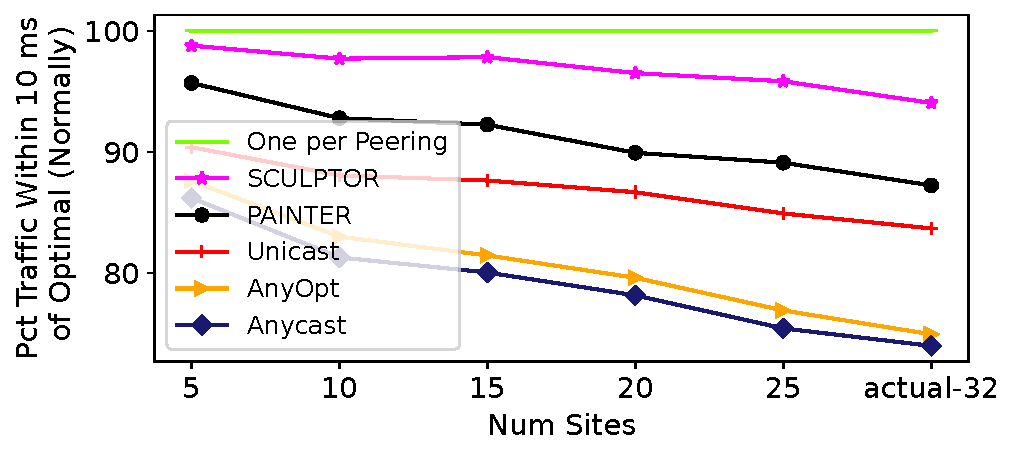
\includegraphics[width=\columnwidth]{figures/percent_traffic_within_10_ms_normal_over_deployment_size.pdf}
        \caption{Normal, 10\,ms.}
    \end{subfigure}~
    \begin{subfigure}{.32\textwidth}
        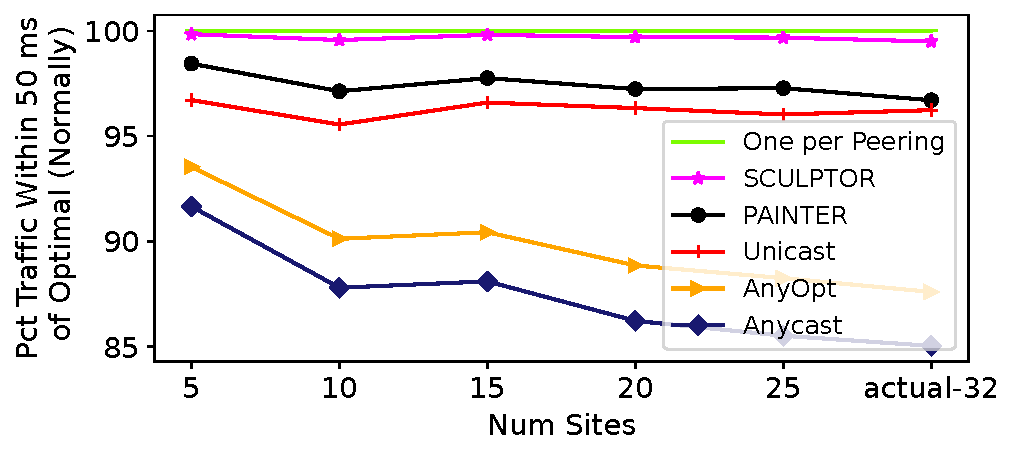
\includegraphics[width=\columnwidth]{figures/percent_traffic_within_50_ms_normal_over_deployment_size.pdf}
        \caption{Normal, 50\,ms.}
    \end{subfigure}~
    \begin{subfigure}{.32\textwidth}
        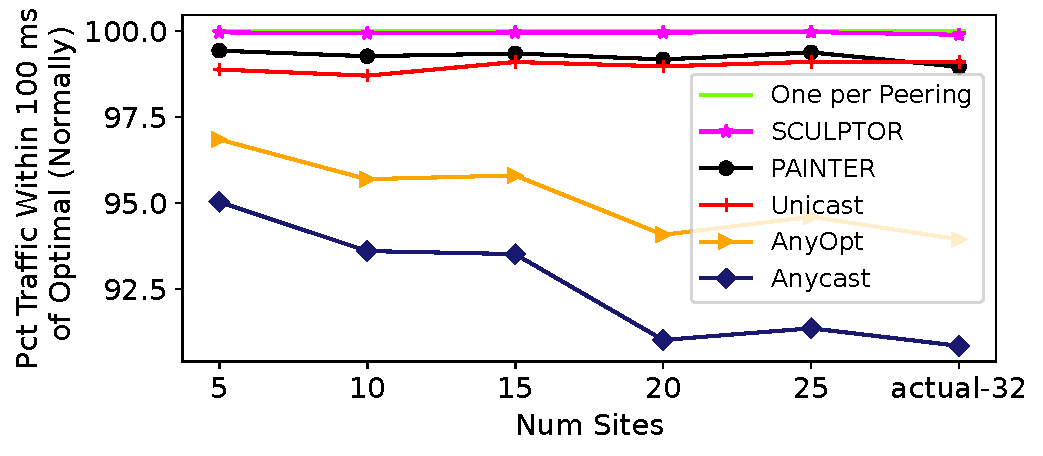
\includegraphics[width=\columnwidth]{figures/percent_traffic_within_100_ms_normal_over_deployment_size.pdf}
        \caption{Normal, 100\,ms.}
    \end{subfigure}\\[.4em]
    \begin{subfigure}{.32\textwidth}
        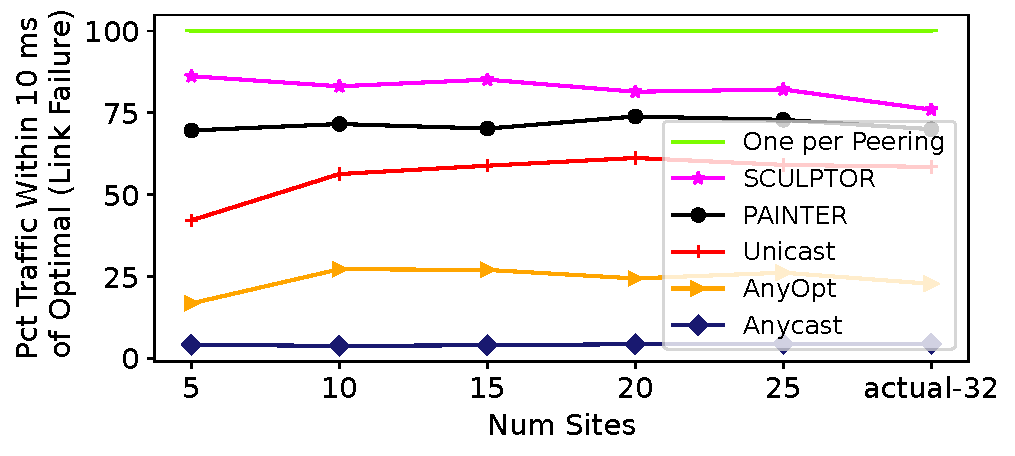
\includegraphics[width=\columnwidth]{figures/percent_traffic_within_10_ms_link_failure_over_deployment_size.pdf}
        \caption{Link failure, 10\,ms.}
    \end{subfigure}~
    \begin{subfigure}{.32\textwidth}
        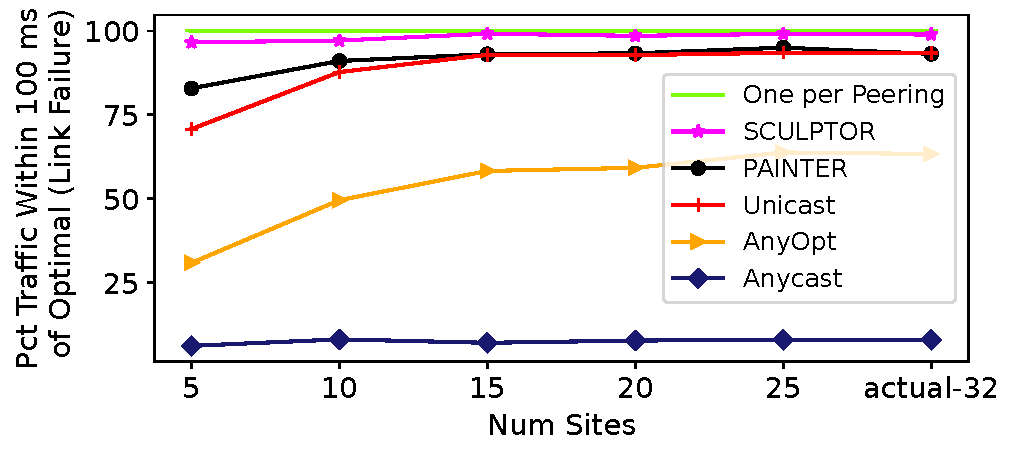
\includegraphics[width=\columnwidth]{figures/percent_traffic_within_100_ms_link_failure_over_deployment_size.pdf}
        \caption{Link failure, 100\,ms.}
    \end{subfigure}~
    \begin{subfigure}{.32\textwidth}
        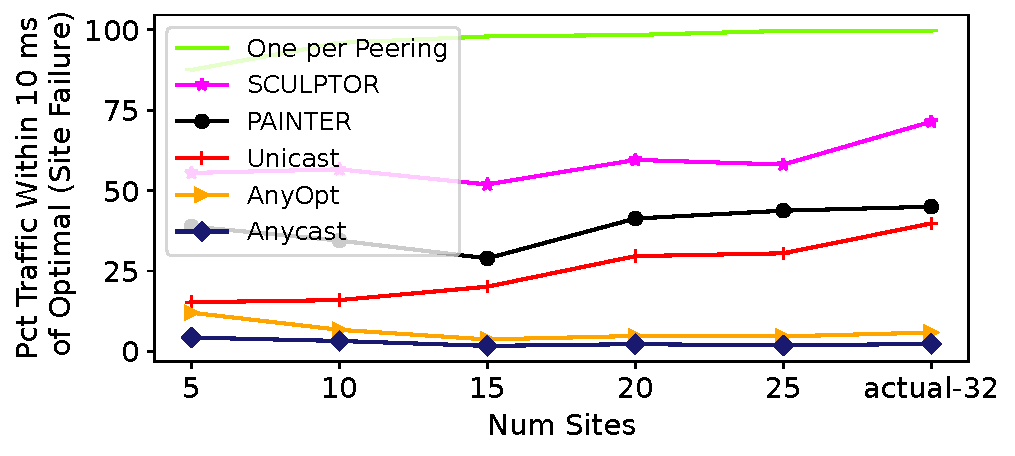
\includegraphics[width=\columnwidth]{figures/percent_traffic_within_10_ms_site_failure_over_deployment_size.pdf}
        \caption{Site failure, 10\,ms.}
    \end{subfigure}
    \caption{Fraction of traffic within tighter and looser latency
        thresholds of \expensive across deployment sizes.  Orderings
        are consistent with the body's $50$\,ms results.}
    \label{fig:additional-thresholds}
\end{figure*}

\begin{figure}[t]
    \centering
    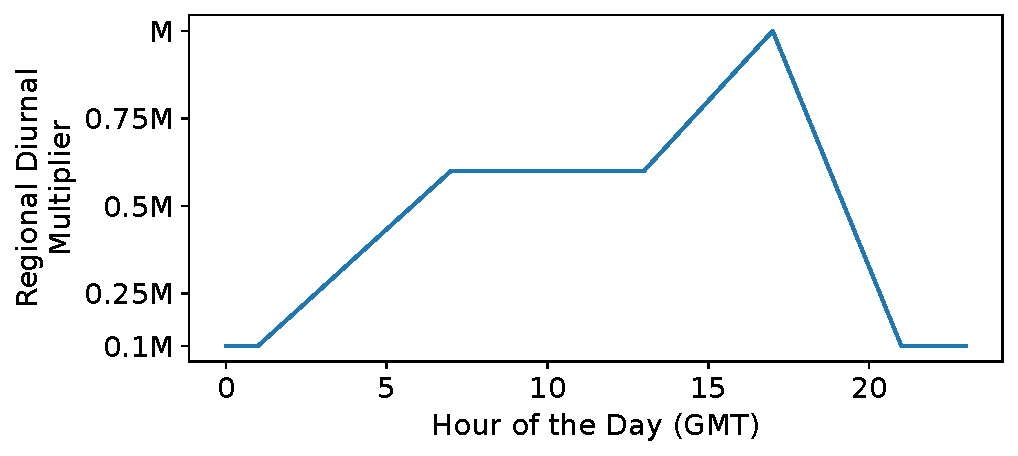
\includegraphics[width=.85\columnwidth]{figures/diurnal_shape.pdf}
    \caption{Diurnal traffic shape used in
        \Cref{fig:infrastructure_utilization_diurnal}, linearly
        interpolated from six points on Edge Node~1's curve in
        Figure~1 of \cite{taiji}.}
    \label{fig:diurnal_shape}
\end{figure}

\end{document}
